\documentclass[12pt]{article}

%%%%%%%%%%%%%%%%%%%%%%%%%%%%%%%%%%%%%%%%%
% Lachaise Assignment
% Structure Specification File
% Version 1.0 (26/6/2018)
%
% This template originates from:
% http://www.LaTeXTemplates.com
%
% Authors:
% Marion Lachaise & François Févotte
% Vel (vel@LaTeXTemplates.com)
%
% License:
% CC BY-NC-SA 3.0 (http://creativecommons.org/licenses/by-nc-sa/3.0/)
% 
%%%%%%%%%%%%%%%%%%%%%%%%%%%%%%%%%%%%%%%%%

%----------------------------------------------------------------------------------------
%	PACKAGES AND OTHER DOCUMENT CONFIGURATIONS
%----------------------------------------------------------------------------------------

\usepackage{amsmath,amsfonts,stmaryrd,amssymb} % Math packages

\usepackage{enumerate} % Custom item numbers for enumerations

\usepackage[ruled]{algorithm2e} % Algorithms

\usepackage[framemethod=tikz]{mdframed} % Allows defining custom boxed/framed environments

\usepackage{listings} % File listings, with syntax highlighting
\lstset{
	basicstyle=\ttfamily, % Typeset listings in monospace font
}

%----------------------------------------------------------------------------------------
%	DOCUMENT MARGINS
%----------------------------------------------------------------------------------------

\usepackage{geometry} % Required for adjusting page dimensions and margins

\geometry{
	paper=a4paper, % Paper size, change to letterpaper for US letter size
	top=2.5cm, % Top margin
	bottom=3cm, % Bottom margin
	left=2.5cm, % Left margin
	right=2.5cm, % Right margin
	headheight=14pt, % Header height
	footskip=1.5cm, % Space from the bottom margin to the baseline of the footer
	headsep=1.2cm, % Space from the top margin to the baseline of the header
	%showframe, % Uncomment to show how the type block is set on the page
}

%----------------------------------------------------------------------------------------
%	FONTS
%----------------------------------------------------------------------------------------

\usepackage[utf8]{inputenc} % Required for inputting international characters
\usepackage[T1]{fontenc} % Output font encoding for international characters

\usepackage{XCharter} % Use the XCharter fonts

%----------------------------------------------------------------------------------------
%	COMMAND LINE ENVIRONMENT
%----------------------------------------------------------------------------------------

% Usage:
% \begin{commandline}
%	\begin{verbatim}
%		$ ls
%		
%		Applications	Desktop	...
%	\end{verbatim}
% \end{commandline}

\mdfdefinestyle{commandline}{
	leftmargin=10pt,
	rightmargin=10pt,
	innerleftmargin=15pt,
	middlelinecolor=black!50!white,
	middlelinewidth=2pt,
	frametitlerule=false,
	backgroundcolor=black!5!white,
	frametitle={Command Line},
	frametitlefont={\normalfont\sffamily\color{white}\hspace{-1em}},
	frametitlebackgroundcolor=black!50!white,
	nobreak,
}

% Define a custom environment for command-line snapshots
\newenvironment{commandline}{
	\medskip
	\begin{mdframed}[style=commandline]
}{
	\end{mdframed}
	\medskip
}

%----------------------------------------------------------------------------------------
%	FILE CONTENTS ENVIRONMENT
%----------------------------------------------------------------------------------------

% Usage:
% \begin{file}[optional filename, defaults to "File"]
%	File contents, for example, with a listings environment
% \end{file}

\mdfdefinestyle{file}{
	innertopmargin=1.6\baselineskip,
	innerbottommargin=0.8\baselineskip,
	topline=false, bottomline=false,
	leftline=false, rightline=false,
	leftmargin=2cm,
	rightmargin=2cm,
	singleextra={%
		\draw[fill=black!10!white](P)++(0,-1.2em)rectangle(P-|O);
		\node[anchor=north west]
		at(P-|O){\ttfamily\mdfilename};
		%
		\def\l{3em}
		\draw(O-|P)++(-\l,0)--++(\l,\l)--(P)--(P-|O)--(O)--cycle;
		\draw(O-|P)++(-\l,0)--++(0,\l)--++(\l,0);
	},
	nobreak,
}

% Define a custom environment for file contents
\newenvironment{file}[1][File]{ % Set the default filename to "File"
	\medskip
	\newcommand{\mdfilename}{#1}
	\begin{mdframed}[style=file]
}{
	\end{mdframed}
	\medskip
}

%----------------------------------------------------------------------------------------
%	NUMBERED QUESTIONS ENVIRONMENT
%----------------------------------------------------------------------------------------

% Usage:
% \begin{question}[optional title]
%	Question contents
% \end{question}

\mdfdefinestyle{question}{
	innertopmargin=1.2\baselineskip,
	innerbottommargin=0.8\baselineskip,
	roundcorner=5pt,
	nobreak,
	singleextra={%
		\draw(P-|O)node[xshift=1em,anchor=west,fill=white,draw,rounded corners=5pt]{%
		Question \theQuestion\questionTitle};
	},
}

\newcounter{Question} % Stores the current question number that gets iterated with each new question

% Define a custom environment for numbered questions
\newenvironment{question}[1][\unskip]{
	\bigskip
	\stepcounter{Question}
	\newcommand{\questionTitle}{~#1}
	\begin{mdframed}[style=question]
}{
	\end{mdframed}
	\medskip
}

%----------------------------------------------------------------------------------------
%	WARNING TEXT ENVIRONMENT
%----------------------------------------------------------------------------------------

% Usage:
% \begin{warn}[optional title, defaults to "Warning:"]
%	Contents
% \end{warn}

\mdfdefinestyle{warning}{
	topline=false, bottomline=false,
	leftline=false, rightline=false,
	nobreak,
	singleextra={%
		\draw(P-|O)++(-0.5em,0)node(tmp1){};
		\draw(P-|O)++(0.5em,0)node(tmp2){};
		\fill[black,rotate around={45:(P-|O)}](tmp1)rectangle(tmp2);
		\node at(P-|O){\color{white}\scriptsize\bf !};
		\draw[very thick](P-|O)++(0,-1em)--(O);%--(O-|P);
	}
}

% Define a custom environment for warning text
\newenvironment{warn}[1][Warning:]{ % Set the default warning to "Warning:"
	\medskip
	\begin{mdframed}[style=warning]
		\noindent{\textbf{#1}}
}{
	\end{mdframed}
}

%----------------------------------------------------------------------------------------
%	INFORMATION ENVIRONMENT
%----------------------------------------------------------------------------------------

% Usage:
% \begin{info}[optional title, defaults to "Info:"]
% 	contents
% 	\end{info}

\mdfdefinestyle{info}{%
	topline=false, bottomline=false,
	leftline=false, rightline=false,
	nobreak,
	singleextra={%
		\fill[black](P-|O)circle[radius=0.4em];
		\node at(P-|O){\color{white}\scriptsize\bf i};
		\draw[very thick](P-|O)++(0,-0.8em)--(O);%--(O-|P);
	}
}

% Define a custom environment for information
\newenvironment{info}[1][Info:]{ % Set the default title to "Info:"
	\medskip
	\begin{mdframed}[style=info]
		\noindent{\textbf{#1}}
}{
	\end{mdframed}
}

\title{VE527: Assignment \#4} % Title of the assignment
\author{Name: Chang Meng\\Student ID:\@\texttt{118370910019}}
\date{\today}

\begin{document}

    \maketitle

    \noindent
    1. (12\%) Given the Boolean function $F(x,y,z,w)=(xy+\overline{x}z)\oplus(wz)$, obtain
    its cofactors $F_x$ and $F_{\overline{y}z}$.

    \noindent
    Answer:

    \noindent
    Let $x=1$,
    \[F_x=(y+0)\oplus(wz)=y\oplus(wz)\]

    \noindent
    Let $y=0$ and $z=1$,
    \[F_{\overline{y}z}=(0+\overline{x})\oplus w=\overline{x}\oplus w\]

    \vspace{12pt}
    \noindent
    2. (12\%) In class, we have shown one form of Shannon expansion:
    \[F(x_1,\dots,x_i,\dots,x_n)=x_i \cdot F(x_i=1)+\overline{x_i}\cdot F(x_i=0)\]
    \noindent
    The above form can be thought of as a "sum of products" form. Actually, there is also a
    "product of sums" of the Shannon expansion:
    \[F(x_1,\dots,x_i,\dots,x_n)=(\overline{x_i}+F(x_i=1))\cdot (x_i+F(x_i=0))\]
    \noindent
    Prove the above "product of sums" expression.

    \noindent
    Answer:

    \noindent
    If $x_i=0$, we have:
    \[
        \begin{split}
            F(x_1,\dots,x_i=0,\dots,x_n) =
            x_i \cdot F(x_i=1)+\overline{x_i}\cdot F(x_i=0) =
            0 + F(x_i = 0) =
            F(x_i=0)
        \end{split}
    \]
    \[
        \begin{split}
            (\overline{x_i}+F(x_i=1))\cdot (x_i+F(x_i=0)) =
            1 \cdot F(x_i=0) =
            F(x_i=0)
        \end{split}
    \]
    \noindent
    If $x_i=1$, we have:
    \[
        \begin{split}
            F(x_1,\dots,x_i=1,\dots,x_n) =
            x_i \cdot F(x_i=1)+\overline{x_i}\cdot F(x_i=0) =
            F{x_i = 1} + 0 =
            F(x_i = 1)
        \end{split}
    \]
    \[
        \begin{split}
            (\overline{x_i}+F(x_i=1))\cdot (x_i+F(x_i=0)) =
            F(x_i=1) \cdot 1 =
            F(x_i=1)
        \end{split}
    \]
    Since the expressions are equal for both $x_i=0$ and $x_i=1$,
    \[F(x_1,\dots,x_i,\dots,x_n)=(\overline{x_i}+F(x_i=1))\cdot (x_i+F(x_i=0))\]

    \vspace{12pt}

    \noindent
    3. (16\%) Consider the small logic network shown below. Obtain the Boolean differences
    $\frac{\partial F}{\partial x}$ and $\frac{\partial F}{\partial y}$.

    \begin{center}
        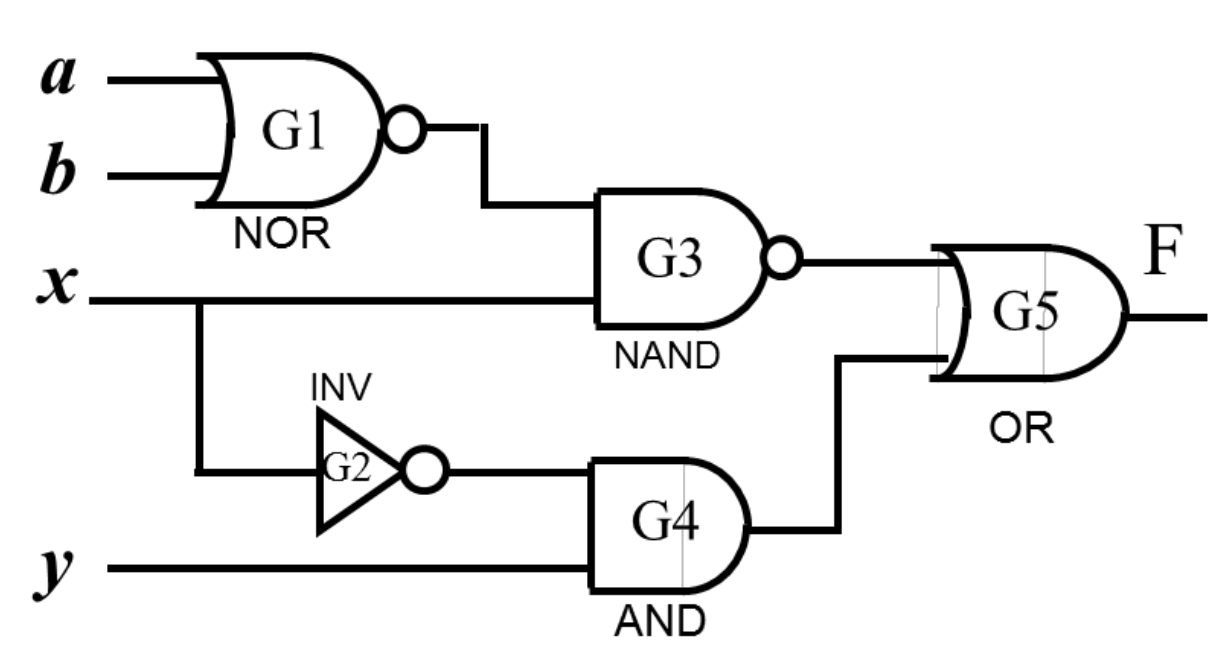
\includegraphics[width = 4.00in, height = 2.20in]{figure1.png}
    \end{center}

    \noindent
    Answer:

    \noindent
    The boolean function of F is:
    \[
        F = \overline{(\overline{a + b}) x} + \overline{x} y
        = a + b + \overline{x} + \overline{x} y
        = a + b + \overline{x}
    \]
    So we have:
    \[
        \frac{\partial F}{\partial x} = (a + b + 1) \oplus (a + b + 0) = 1 \oplus (a + b)
        = \overline{a + b}
    \]
    \begin{center}
        $\frac{\partial F}{\partial y} = 0$, because $F$ is not relevant to $y$.
    \end{center}

    \noindent
    4. (10\%) For the logic network from Problem 3, obtain the universal
    quantification ($\forall{x} F$) and the exisitential quantification
    ($\exists{x} F$).

    \noindent
    Answer:
    \[ \forall{x} F = F_x \cdot F_{\overline{x}} = (a + b) \cdot 1 = a + b \]
    \[ \exists{x} F = F_x + F_{\overline{x}} = a + b + 1 = 1 \]

    \noindent
    5. (24\%) Network repair.

    \noindent
    The carry output of a 1-bit adder has the Boolean function $c_{out} = ab + (a + b)c_{in}$,
    where $a$ and $b$ are the 1-bit numbers we want to add, and $c_{cin}$ is the input carry
    bit. The figure below shows an implementation of the above function. However, the
    implementation is not correct. We suspect that the gate the the "??" label is incorrect.
    Use the logic network repair procedure discussed in the lecture to fix the suspicious
    gate. What could this gate be?

    \begin{center}
        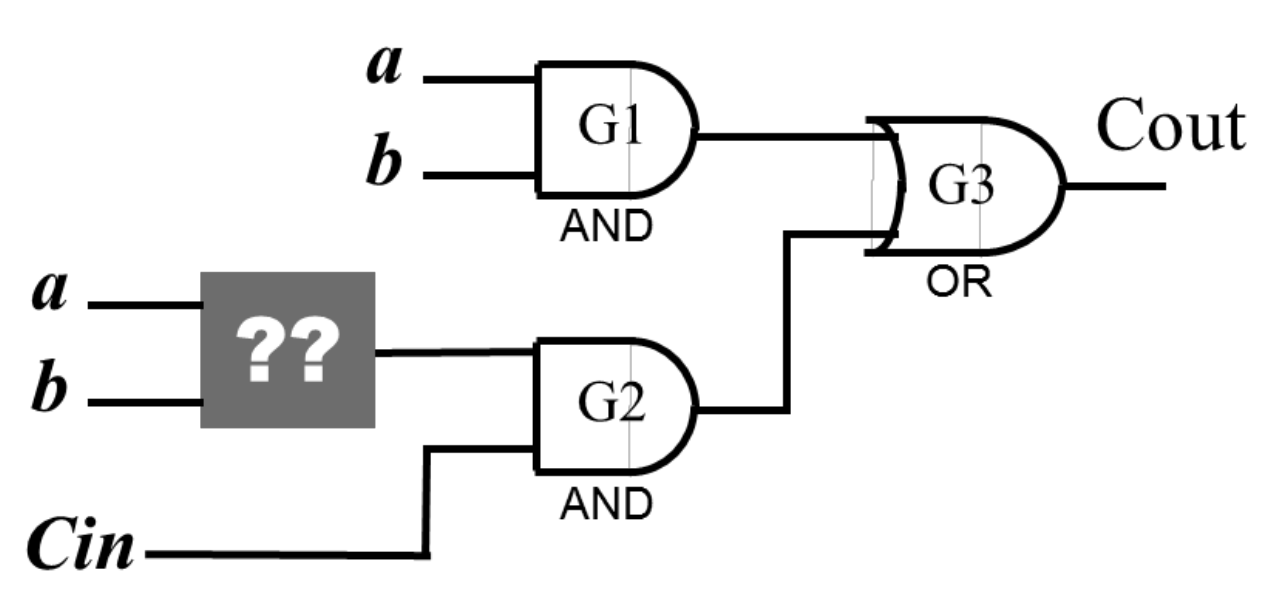
\includegraphics[width = 4.00in, height = 1.80in]{figure2.png}
    \end{center}

    \noindent
    Answer:

    \noindent
    We see the suspicious gate as a 4-to-1 MUX, the output of MUX $f$ is:
    \[ f = d_0 \overline a \overline b + d_1 \overline a b + d_2 a \overline b + d_3 a b \]
    \noindent
    Then we can calculate the output $G$:
    \[ G1 = ab \]
    \[
        G2 = f c_{in} =
        c_{in} (d_0 \overline a \overline b + d_1 \overline a b + d_2 a \overline b + d_3 a b)
    \]
    \[
        G = G1 + G2 =
        ab+c_{in}(d_0 \overline a \overline b+d_1 \overline a b + d_2 a \overline b + d_3 a b)
    \]
    \noindent
    By xnor $G$ with the given $c_{out}$ function, we get:
    \[
        z = G \overline{\oplus} c_{out} =
        (ab+c_{in}(d_0 \overline a \overline b+d_1 \overline a b+d_2 a \overline b+d_3 a b))
        \overline{\oplus} (ab + (a + b)c_{in})
    \]
    \noindent
    To repair it, we should find values of $d_0$, $d_1$, $d_2$, $d_3$ so that:
    \[
        (\forall{abc_{in}}\ z)(d_0, d_1, d_2, d_3) =
        z_{\overline a \overline b \overline c_{in}} \cdot
        z_{\overline a \overline b c_{in}} \cdot
        z_{\overline a b \overline c_{in}} \cdot
        z_{\overline a b c_{in}} \cdot
        z_{a \overline b \overline c_{in}} \cdot
        z_{a \overline b c_{in}} \cdot
        z_{a b \overline c_{in}} \cdot
        z_{a b c_{in}} = 1
    \]
    \noindent
    So values of every z's cofactor are 1.
    \[
        z_{\overline a \overline b \overline c_{in}} =
        G_{\overline a \overline b \overline c_{in}} \overline \oplus
        c_{out,\overline a \overline b \overline c_{in}} = 1
    \]
    \[
        z_{\overline a \overline b c_{in}} =
        G_{\overline a \overline b c_{in}} \overline \oplus
        c_{out,\overline a \overline b c_{in}} = \overline{d_0} = 1,
        d_0 = 0
    \]
    \[
        z_{\overline a b \overline c_{in}} =
        G_{\overline a b \overline c_{in}} \overline \oplus
        c_{out,\overline a b \overline c_{in}} = 1
    \]
    \[
        z_{\overline a b c_{in}} =
        G_{\overline a b c_{in}} \overline \oplus
        c_{out,\overline a b c_{in}} = d_1 = 1
    \]
    \[
        z_{a \overline b \overline c_{in}} =
        G_{a \overline b \overline c_{in}} \overline \oplus
        c_{out,a \overline b \overline c_{in}} = 1
    \]
    \[
        z_{a \overline b c_{in}} =
        G_{a \overline b c_{in}} \overline \oplus
        c_{out,a \overline b c_{in}} = d_2 = 1
    \]
    \[
        z_{a b \overline c_{in}} =
        G_{a b \overline c_{in}} \overline \oplus
        c_{out,a b \overline c_{in}} = 1
    \]
    \[
        z_{a b c_{in}} =
        G_{a b c_{in}} \overline \oplus
        c_{out,a b c_{in}} = 1
    \]
    We have $d_0 = 0, d_1 = 1, d_2 = 1, d_3 = X$, the gate could be OR, XOR.

    \vspace{12pt}
    \noindent
    6. (10\%) Suppose we have the following cube-list at one node of our URP tautology
    recursion, and we need to decide on splitting variable to use to cofactor and recurse.
    Which variable will you pick, and why?
    \[
        \begin{matrix}
            x & y & z & w \\
            11 & 01 & 01 & 11 \\
            01 & 11 & 10 & 01 \\
            01 & 10 & 11 & 11 \\
            10 & 11 & 10 & 10 \\
            01 & 11 & 01 & 10
        \end{matrix}
    \]

    \noindent
    Answer:

    \noindent
    $x$, $y$, $z$, $w$ has 4, 2, 4, 3 product dependent terms separately, we should pick one
    from $x$ or $z$.

    \noindent
    The value of $|\#true\_var - \#compl\_var|$ of $x$, $z$ is 2, 0 separately. So we pick $z$
    for balance.

    \vspace{12pt}
    \noindent
    7. (16\%) For the cube-list from Problem 6, suppose we choose the splitting variable as
    $w$. What are the resulting cube-list for its positive and negative cofactors,
    respectively?
    \noindent
    Answer:

    \noindent
    Positive cofactor:
    \[
        \begin{matrix}
            x & y & z & w \\
            11 & 01 & 01 & 11 \\
            01 & 11 & 10 & 11 \\
            01 & 10 & 11 & 11
        \end{matrix}
    \]
    Negative cofactor:
    \[
        \begin{matrix}
            x & y & z & w \\
            11 & 01 & 01 & 11 \\
            01 & 10 & 11 & 11 \\
            10 & 11 & 10 & 11 \\
            01 & 11 & 01 & 11
        \end{matrix}
    \]

\end{document}
